\chapter{Background}
\label{chap:background}

As discussed in Chapter \ref{chap:introduction}, a simple robot learning algorithm will allow the agent to generalise to different environment setups.
There are three main techniques which allow us to achieve this, however each of these methods come with some major drawbacks which will be discussed.

\section{Model Based Control}
\label{sec:model-based-control}
In this first method, in order to teach the robot how to complete the desired task, the human needs to provide to the robot a model of the environment and a reward function \cite{model-based-control}. The model is a function which encapsulates the dynamics of the environment, and the ways that actions influence the state. Specifically, it is a map from the current state and chosen action to the resulting next state:
$$\mathcal{P} : \state \times \action \mapsto \state$$

The reward function is some function which maps the current world state and action chosen by the agent to a real number:
$$\reward : \state \times \action \mapsto \real$$

Here $\state$ denotes the set of all possible states the system can be in, and $\action$ denotes the set of all possible actions the robot may take.\\

The robot then tries its best to maximise this reward by choosing the actions which give a high reward now, but that also lead to states with the potential to yield high rewards later. It is able to predict which states it will reach later using the environment model. The priority between getting an immediate reward now and ensuring higher rewards later is controlled through the discount factor $\gamma \in [0,1]$. If the robot is provided with these aspects, and the model perfectly captures the environment dynamics , then the robot can directly solve the induced Markov Decision Process (MDP), for example using a dynamic programming approach to calculate the expected rewards of being in every state \cite{rl-intro-book}. Then the agent can simply take the actions which ensures it follows the sequence of states with highest expected rewards.\\
%TODO: cite , dynamic programming, bellman equations

Referring back to the success criteria questions mentioned in \refchap{chap:introduction}, this method teaches the robot \speech{How do I know when I have completed the task?} The task is completed when this given reward function is maximised. It is up to the engineer to ensure that this reward function really does capture the specifics of the underlying task, since the robot has no true understanding of the task. The robot is merely trying to maximise a number, wherein it has been told that getting the number as big as possible, will complete the task. We have also implicitly defined \speech{What does it mean to complete the task?} To complete the task is to score highly in the reward function.\\

The problem with this method is it is a lot of work to design the reward function and environment model. In some cases the environment may not even be fully observable. As such a complete model is simply not possible. As a result Model based control is most often used in specific lab settings where the environment can be meticulously controlled. It is rarely used in so called \socalled{in the wild} robot learning due to the inability to guarantee control over the environment, resulting in an unreliable environment model. As such, Model Based Control lacks the generalisability we strive for in this paper, and so will not be considered further.

\section{Reinforcement Learning}
\label{sec:reinforcement-learning}
The second method at our disposal is Reinforcement Learning \cite{rl}. In this method we do not need to provide the agent a model of the environment. However, the agent still requires a reward function. The robot will explore the environment on its own to experience states and see which ones yield high rewards \cite{rl-intro-book, rl-book}. After sufficiently long training, the robot's ideas of which states have a high associated reward should approach the true values. These values were known outright in Model Based Control thanks to the environment model, however in Reinforcement Learning the agent explores the state space itself to approximate these values. The robot is then able to select the actions which lead to states it has experienced giving high rewards.\\

This method answers the success criteria questions in exactly the same way as with Model Based Control. The reward function still solely encodes information as to the completion of the task. The only difference is in how much information the robot has available to pursue improving the reward function, and hence completing the task. Instead of a perfect understanding of the world and how these interactions affect the reward function, the robot only has information it has experienced itself.\\

While this method is a big improvement over model based control, there is still a problem. We still need to provide the agent a reward function. This can be difficult to formulate, even more so without the environment knowledge of model based control. When we had access to the environment model we had knowledge of the relative positions of objects, and could easily define tasks which involved moving one object to another place. For example the reward function could be the negation of the distance between the object's position and the target position. Alas, without the environment model, the agent cannot know perfectly the position of the objects and the target position. These must be estimated from the environment observations it makes. Such observations are usually in the form of a camera attached to the robot, often mounted in a fixed third person view, or mounted on the wrist for a first person view. From these observations, the robot can estimate the position of objects, given their position in the image, and the known position of the camera when the image was taken.\\

Despite only having access to estimates through observations, carefully designing a reward function is a reasonable approach. The issue comes with the increased workload of a generalisable system. If we wish to teach the agent multiple tasks we are required to provide the agent one reward function for every task we wish it to complete. Furthermore, we need some way to decide which task to complete and select the correct reward function. Since each task may be wildly different, it is simply not possible to encode all of these tasks with a single reward function. As such, Reinforcement Learning is more applicable to fine tuning a solution to a specific task. Since the robot explores the environment itself, there is little bias to the solution, given the robot explores sufficiently within the state space. This is desirable for finding optimal solutions to a problem that the engineers may not have considered. As we will see in the next section, other solutions often introduce large amounts of human bias to the solutions the robot finds. However, poor exploration from the robot can lead to sub-optimal results, if the agent gets stuck exploiting a local optima, when it could have reached a better solution by exploring further. This tendency to get stuck with a sub-optimal solution is obviously undesirable. \\

It can be difficult to decide a strategy for this \socalled{exploration vs exploitation} problem. A high exploration means the agent can in theory experience more of the state space. However, the exploration can be very unfocused, leaving the robot exploring an area which is not likely to yield good results. Exploitation refers to the agent choosing the best action it can at its current state. A good algorithm balances some exploitation to keep the robot focused in the direction of the currently believed best solution, while allowing exploration to test out close by states, which are more likely to perform well. This balance is often achieved through \socalled{epsilon-greedy exploration}, wherein $\epsilon$ is a hyperparameter probability. The agent will choose the greedy option, the best currently known action in its current state, with proportion $\epsilon$. Otherwise it will choose any other random action with probability $1-\epsilon$. When choosing the random action, all actions are drawn from a uniform distribution. Choosing a good value for this hyperparameter is difficult and largely dependent on the specific problem environment. Additionally, this all assumes the environment is continuous, meaning that near by states behave similarly to their neighbours. If this is not the case, then keeping the exploration focused about the current optimal solution, offers little benefit.

\section{Imitation Learning}
\label{sec:imitation-learning}
With these issues in mind, the third common robot learning method is Imitation Learning. This method attempts to simplify the data collection required of the engineers and reduce the impact of hyperparameters. Instead of needing to provide a reward function to the agent, we instead provide demonstrations of how to complete the task. The key paradigm shift is that rather than telling the robot what we want it to do (through the reward function) and leaving it to work out how to do that, we instead show the robot exactly how to perform a task. This generally gives a much faster return on investment since the robot is immediately able to perform the task somewhat well, as opposed to learning an optimal solution through time consuming exploration in the environment. This does however, have a few downsides. Most notably we, the engineers, need to be able to perform the task ourselves. We cannot teach the robot to perform a task if we fail to show it a successful demonstration. Furthermore, the robot's solutions are heavily biased towards the human demonstrations. The agent will not do much exploring and innovating on the solutions presented by the humans. Depending on the implementation the agent may process the provided demonstrations differently.

\subsubsection{Inverse Reinforcement Learning}
One approach is to use Inverse Reinforcement Learning to infer the reward function from the provided demonstrations \cite{inverse-rl}. We may use a function approximator, such as a neural network to replace the reward function. Given the robot's state and chosen action, we want the approximator to output the reward for this action. In this scenario we use the demonstrations, along with associated, presumably high rewards to train this network. For example, stating that all human demonstrations receive a fixed reward of 100, since they accomplish the task. With a reward function now known, the agent can use the previously discussed forward Reinforcement Learning to solve the task in similar situations.\\

In this implementation we attempt to again teach the robot \speech{How do I know when I have completed the task?} The difference being how we convey this to the agent. We give the robot a number of demonstrations which are considered as successful completions of the task. From this the robot tries to infer what was common about all these demonstrations which makes them successful at completing the task. The difficulty lies in the fact that often very many reward functions could explain the behaviour. Was the task to grasp the mug or to just move the end effector to the right? To us it may seem obvious that it was probably the first option, but to the robot both of these options are valid.

\subsubsection{Behavioural Cloning}
Another approach is to forgo the reward function entirely. In Behavioural Cloning \cite{behavioural-cloning, behavioural-cloning-book}, the agent instead uses the demonstrations as a blueprint to follow. Similar to Inverse Reinforcement Learning, we will still train a function approximator. However this time we will be using it as the robot's policy, not the reward function. The approximator will take in the robot's current state (or an observation of the state if it is not fully observable), and predict the optimal action. This approximator is trained on the demonstrations so that for each state in the demonstration, the ground truth output is the action which the human took in the demonstration.\\

In this implementation we are changing how we answer the success criteria questions. This time we are directly teaching the robot \speech{What does it mean to complete the task?} We are teaching the robot exactly how we as humans would solve this task. In this method the robot never gets an answer to the question \speech{How do I know when I have completed the task?} The robot has no actual concept of what it is doing and how to know when it succeeds. All it knows is \speech{This is what the human did, so I should do that too.} It trusts that the demonstrations it has been given, will allow it to complete the task.

\subsection{Training data problem}
Both of these approaches to Imitation Learning require a large diverse set of demonstrations. This is because we use the demonstrations to train a neural network. As such we need lots of training data in order to expect the function approximators to produce reasonable results. The trade off is that instead of providing a single but complicated and hard to craft reward function, we instead need to supply many simple to collect demonstrations. Although note that simple does not necessarily imply easy. While the collection of demonstrations can be straight forward, either through teleoperation (remote controlling the robot) or kinesthetic demonstration (physically moving the robot yourself), we need to provide a large amount of them which can be time consuming.\\

The additional complexity of providing demonstrations is hidden in the fact that for the agent to learn effectively, the demonstrations must be of high quality. For example, we need to ensure the demonstrations actually accomplish the goal, otherwise the robot will likely also fail to achieve the goal. Since the robot does not have a reward function, it has no way to evaluate which demonstrations were good. It instead treats all demonstrations equally, trusting that they achieve the same thing we want the robot to achieve. If a demonstration slightly misses the goal, the robot may think that this near miss state, is actually the true goal state. Problems like this one make the agent very sensitive to the initial conditions, since poor quality demonstrations may prevent it from learning anything.

\subsection{State distribution problem}
Another complication is that we need the demonstrations to be diverse so that a wide variety of states are reached. If the demonstrations do not sufficiently cover the state space the robot will be operating in, then the robot will likely find itself in a state for which it has no information how to proceed. In this scenario it is likely to perform an action which seems random. This is simply because function approximators struggle to extrapolate to inputs which are out of distribution. If we want our agent to know what to do in a wide variety of states it may find itself in, then we need to show it how to handle these states, by making sure our demonstrations at some point visit these states.\\

Ensuring the demonstrations cover the state space the robot will be experiencing during testing is a difficult problem. Simply because we cannot know for sure which states the robot will need to traverse in order to reach the goal. While providing a diverse set of demonstrations is a good start, it is always possible the robot will find itself in a state for which it does not know how to proceed. \socalled{DAgger} (Dataset Aggregation) is a Behavioural Cloning technique which aims to solve this problem \cite{dagger}. In this algorithm the agent determines its policy to complete the task, then for every state along this trajectory, the system requests a demonstration from the human. This demonstration shows what the human would have done to complete the task, from this state. This ensures that we provide demonstrations for states which the robot actually visits. There are two main problems with this design. Firstly, we cannot pre-collect all the demonstrations. The robot will propose a policy, and then request more training demonstrations. The agent then needs to retrain the policy on this new training data, taking more time. This means the training time is interleaved with the test time. A preferable design would allow us to collect all the demonstrations up front, and then test the agent with no further demonstrations required. The second problem is the sheer volume of required demonstrations. DAgger requires us to collect one full demonstration from every state along the proposed trajectory. This means the number of required demonstrations is dependent on the length of the trajectory. If the environment involves a continuous state space or a task involves a very long and complex trajectory, then this increases the demonstration burden even further.\\

Alternatively, rather than requesting a demonstration for every state along the trajectory, we can instead request a demonstration only when the robot is unsure what it should do. This is a strategy employed by \socalled{Uncertainty-Based Imitation Learning} \cite{uncertainty-il}. While this still has the issue of mixing the testing and training time, it requires far less demonstrations overall than DAgger. We may use any method of quantifying uncertainty within the robot's actions. One such approach is to use an ensemble of policy networks. Each network is trained on a subset of the training data, and when the predictions of optimal action differ wildly between each network, it means the agent is unsure what to do.

\subsection{Reducing the dependency on demonstrations}
\label{subsec:one-shot}
While these previously stated methods help to ensure the demonstrations are diverse, they achieve this by collecting far more demonstrations overall. The requirement to collect a large set of human provided demonstrations is the main bottleneck in an Imitation Learning system as it is a time consuming process. We wish to reduce the requirement for large amounts of training data by leveraging alternative approaches to generalise the demonstrations.\\

The work of A. Mandlekar et al. \cite{mimicgen} proposes a system to upscale a small number of demonstrations into a larger set. Their system, \socalled{MimicGen}, takes as input a small number of human provided demonstrations. It then segments these demonstrations into \speech{object centric subtasks} and constructs new ones by stitching together subtasks. MimicGen also transforms the scene so that each demonstration is diverse in positioning. This system reduces the burden of collecting demonstrations since we now need to collect far fewer demonstrations and can simply up-sample to a larger dataset. In the paper they claim \speech{Image-based agent performance is comparable on 200 MimicGen demos and 200 human demos, despite MimicGen only using 10 source human demos.} This means we could collect only 10 demonstrations, up-sample to 200 using MimicGen and have the same accuracy as if we collected 200 demonstrations manually. This dramatically reduces the workload of collecting demonstrations.\\

Another approach to solve the need for a large set of demonstrations is to provide the agent with alternative information to allow it to generalise to unseen environments thus removing the need for a large dataset of demonstrations entirely. The logical progression of this idea is to reduce the demonstration burden on the engineers as far as possible. So called \socalled{one-shot} algorithms stand as the pinnacle of this design philosophy, by allowing the robot to learn a given task from only a single human provided demonstration.\\

Specifically, P. Vitiello, K. Dreczkowski and E. Johns utilise an RGB-D image of the environment before the demonstration in their paper titled \speech{One-Shot Imitation Learning: A Pose Estimation Perspective} \cite{one-shot-pose-estimate}. This paper creates a system which upon being presented with a new scene, takes a similar picture of this new environment. The system then calculates the transformation which maps the object of interest in the demonstration to its position in the new environment. For example the system may notice by comparing the two images that the object of interest has moved 10cm to the left and rotated 30 degrees clockwise about the Z axis. The agent then applies this same transformation to the robot pose in the demonstration trajectory. The effect of this is to transform the positions at each time step so that the robot will move to a position 10cm to the left with a 30 degree clockwise rotation when compared to the original demonstration. Conceptually what this does is map the demonstration from the old environment to the new one. Now that the demonstration has been mapped to the new environment, the agent can simply execute the transformed demonstration, which will complete the task. The above solution manages to drastically reduce the workload of collecting demonstrations for the imitation learning task. As the name \speech{One-shot imitation learning} suggests, only a single demonstration is required. Furthermore, the additional information required by the agent, the \speech{context vector} as this paper calls it, can be collected automatically by the agent during the demonstration with no additional human input needed.\\

N. Di Palo and E. Johns propose a similar method \cite{one-shot-imitation} which uses a wrist mounted camera as opposed to the previous solution which utilised a third person camera which captured the entire scene. The advantage of a wrist mounted camera is that the camera is moving with the end effector. This effectively makes the image captured translation and rotation invariant relative to the end effector pose. The only important information is the relative pose between the end effector and the object in the scene. The advantage of this is that we reduce the need for complicated computer vision methods for pose estimation of the objects between the two images \cite{one-shot-pose-estimate}. In the work by N. Di Palo and E. Johns, since the camera moves with the end effector, changes in the end effector position and orientation are reflected very obviously in the captured image \cite{one-shot-imitation}. This also means that the agent simply needs to line up the end effector so that the captured image is the same as the demonstration image. If this is the case then the relative position between the end effector and the object is the same as in the demonstration. As such the current position and orientation of the end effector after lining up but before starting the task, can be calculated using forward kinematics and added as an offset to the poses in the demonstration. As before, this transformed trajectory can now be executed which will execute the task as in the demonstration, but mapped into the new scene.\\

Another advantage is that a wrist mounted camera also reduces the noise within the image. A third person camera which captures the entire scene will capture all objects within the scene, even though only one may be of relevance to the task. This additional noise could cause the agent to incorrectly compute the transformation between the demonstration and current scene, and therefore fail the task. Alternatively, a wrist mounted camera will only capture the focused view around the end effector. This means that during the manipulation task, the object of interest will likely be the only object within the image. This focused view is much less susceptible to noise of other objects within the environment.\\

There are of course, as with every design decision, some drawbacks to using a wrist mounted camera. Most obviously, due to the focused view failing to capture the entire scene, it can be difficult to locate the object of interest. This means that a single image may no longer be enough as the object we are looking for may not be present in the image if the camera is pointing the wrong way. This necessitates a live feed of the wrist mounted camera as opposed to the single image capabilities of the third person camera, which is a major drawback.\\

The other large drawback is a consequence of this first one. Since a live feed of the image is now required, any objects blocking the camera will now cause a serious problem. This was not an issue with the third person camera as it could capture the entire scene and everything it needed to know before starting to execute the task. However with the wrist mounted camera, if the robot picks up an oddly shaped object which happens to block some or all of the image feed, then the robot will quite literally be executing the task blind. This is not such a problem for tasks involving a single object of interest, since it is assumed the robot can navigate the arm and line up with the demonstration image while no object is in its gripper, and therefore nothing should be blocking the camera. The real problem comes with multi-stage tasks.
Consider the task which is to pick up a spoon and place it in a mug. The demonstration would pick up the spoon from a particular position and angle relative to the spoon. It would then move to a particular position and angle relative to the mug and release the spoon from its gripper. Now suppose the agent is deployed on a new task with a slightly bigger spoon, and the spoon and mug rearranged. The agent would be able to find the spoon, move to a relative position which matches as in the demonstration, and execute the trajectory to pick up the spoon. However, since the task involves two objects, we can no longer just execute the entire demonstration from this point, since the relative position between the spoon and the mug may have changed. As such we need to partition the trajectory and line up the end effector relative to the object of interest for each segment. It is clear to see that the trajectory can be segmented every time the object of interest changes \cite{mimicgen}. This itself generally happens when the gripper closes, picking up the previous object of interest, or when the gripper opens, placing the grasped object in a position relative to the current object of interest. In this example initially the object of interest is the spoon, we move relative to the spoon and execute the segment of the demonstration which picked up the spoon. Now that the spoon is attached to the end effector, the object of interest is now the mug. We want to move to a position which is relative to the mug, the same as in the demonstration. At this point we can execute that segment of the trajectory to drop the spoon. This system works fine given that the camera is a live feed and so we can keep checking the relative position of the end effector to the object we currently care about. The issue however, comes when the object in the gripper is obstructing the view of the camera. If this slightly larger spoon is now blocking the camera, the agent will be unable to find the mug and line up relative to it. In this scenario there is nothing the robot can do. It needs the spoon in its gripper to progress to the next segment of the demonstration, but when it is holding the spoon it cannot see the environment. The robot is unable to know its location relative to the mug, so cannot progress with the next segment. This demonstrates the issue with a wrist mounted camera. There are some objects which when picked up will block the camera, and there is very little the robot can do to work around this. There are just some objects the agent cannot deal with. The affects of this issue can be mitigated by careful placement of the wrist mounted camera. Placing it further up the wrist away from the end effector makes it less prone to being blocked by the object in the gripper. While this is potentially a big problem, it is unlikely that this will happen in practice. This issue could be further prevented by utilising two cameras, perhaps one on each side of the wrist, reducing the chance that an object would block both cameras, rendering the robot blind again. Of course with all these solutions, a contrived scenario with an object shaped perfectly to block the cameras will cause problems. However with everyday regular items, the affects of this problem should be limited.\\

Having reviewed the current literature, we now cover some preliminary knowledge which will be necessary in understanding the system we develop in this paper.

\section{Preliminaries: Rotations and Orientations}
\label{sec:rotations}
Throughout this report best effort will be made to not confuse the terms \socalled{rotation} and \socalled{orientation}. While mathematically these terms are represented identically, they have different semantic interpretations. As such the language within this paper will be consistent with the following definitions:\\
A \textbf{rotation} is a function which refers to the circular movement of an object around a central point or axis.\\ %TODO come up with better def of rotation
An \textbf{orientation} is an angular displacement relative to an agreed upon reference frame. It is the resulting state after a rotation is applied to a body which was initially in the starting reference frame. Typically the base orientation will be such that the object's local coordinate frame aligns with the world coordinate frame. The object's orientation is then the rotation about the object's local origin, which aligns the world reference frame with the object's local reference frame.\\

From these definitions we can realise that to find an object's new orientation following a rotation, we compose the applied rotation with the object's previous orientation. This results in the total rotation which maps the object from the base reference frame to its new local frame, which is by our definition, its new orientation.\\

\begin{figure}[h]
    \centering
    \begin{subfigure}[b]{0.45\textwidth}
        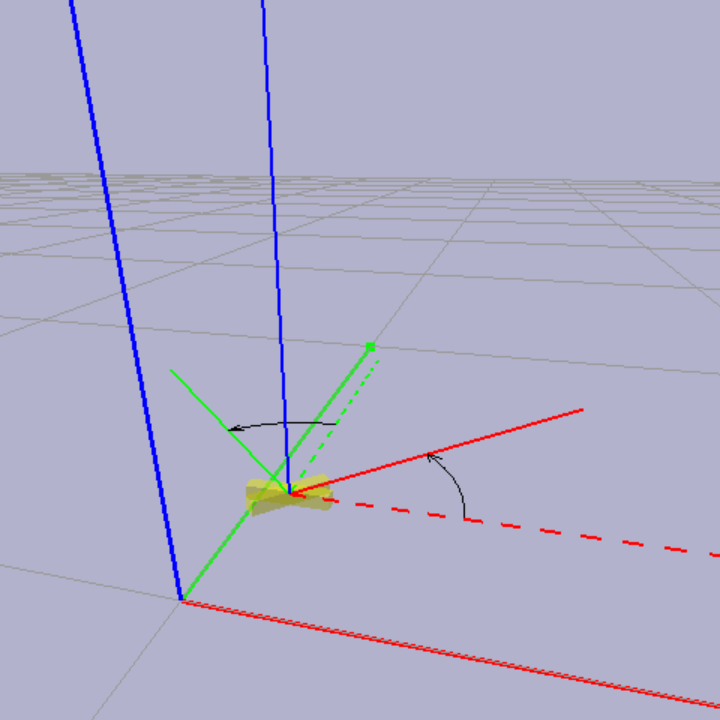
\includegraphics[width=\textwidth]{figures/coordinate_figure1.png}
    \end{subfigure}
    \hfill
    \begin{subfigure}[b]{0.45\textwidth}
        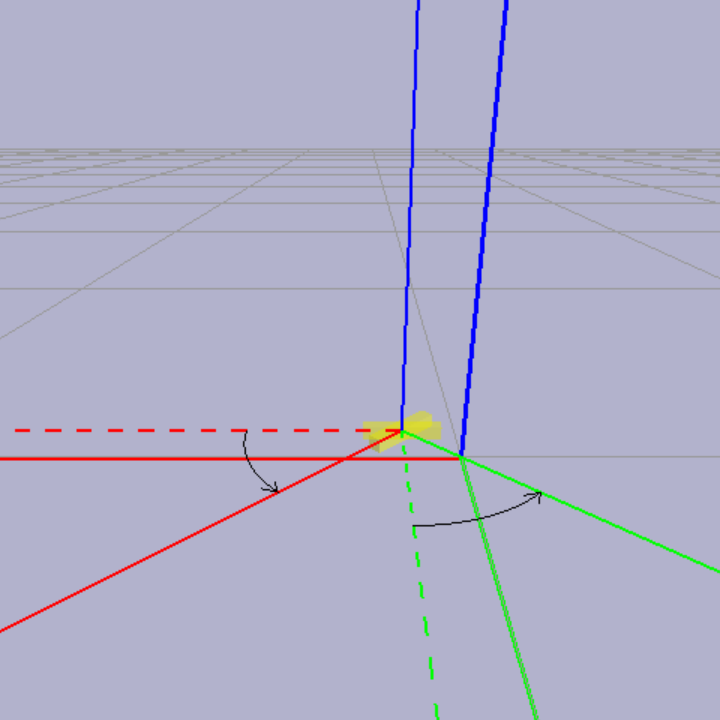
\includegraphics[width=\textwidth]{figures/coordinate_figure2.png}
    \end{subfigure}
    \caption[An object before and after a rotation of $\frac{\pi}{4}$ about the Z axis]{An object before and after a rotation of $\frac{\pi}{4}$ about the Z axis \footnotemark}
    \label{fig:orientations}
\end{figure}
\footnotetext{Refer to \refsubsec{subsec:right-hand-rule} for an explanation on rotation direction}
%TODO latex flags an error but it seems fine. Double check figure and footnote are fine before submission

\reffig{fig:orientations} showcases an object in two different possible orientations. The dotted lines show the object's local coordinate frame prior to the object being rotated. We can see that the dotted coordinate frame aligns with the world coordinate frame, just translated by the object's position. As such we define this orientation as the initial frame of reference. Therefore we would choose to encode this orientation as the identity rotation since no rotation is needed to align the world frame with the object's local frame.\\

The solid line coordinate frame shows the object's local coordinate frame after it has been rotated $\frac{\pi}{4}$ radians about the Z axis \textit{from the initial frame of reference}. Therefore we represent this orientation with the rotation $\frac{\pi}{4}$ radians about the Z axis. It would be equally valid to encode this as the rotation matrix, Euler angles or any other encoding of this rotation, but we will see in the next subsection that the method used in this project is quaternions. \reffig{fig:orientations} shows the exact same setup from two different view points, to better visualise the rotation described.

%Given this project focuses on manipulating objects in 3D space, it would be pertinent to understand the main way these rotations and orientations are encoded in our system.
\subsection{Quaternions}
\label{subsec:quaternions}
Quaternions are a 4 dimensional number system \cite{quaternions} which can be used to represent and manipulate orientations and rotations in 3D space \cite{orientations}. In many ways they are an extension of the complex numbers, adding an additional 2 complex axes. A quaternion consists of a real component and 3 imaginary components which are often grouped together and called the vector component.
$$q \in \quat, \longspace q = a + b\qi + c\qj + d\qk, \longspace where \: \: a,b,c,d \in \real$$
The fundamental imaginary units follow the set of rules listed below:
\begin{itemize}
    \item $\qi \neq \qj \neq \qk$
    \item $\qi^2 = \qj^2 = \qk^2 = \qi\qj\qk = -1$
    \item $\qi\qj = \qk, \shortspace \qj\qi = -\qk$
    \item $\qj\qk = \qi, \shortspace \qk\qj = -\qi$
    \item $\qk\qi = \qj, \shortspace \qi\qk = -\qj$
\end{itemize}

Of relevance to us however, is how these numbers can represent 3D rotations. If we consider a rotation in axis-angle form, that is that we rotate some angle $\theta$ about some normalised unit vector $v = (x,y,z)$, then we can produce the unit quaternion:
% $$q = \cos{\frac{\theta}{2}} + x\qi \sin{\frac{\theta}{2}} + y\qj \sin{\frac{\theta}{2}} + z\qk \sin{\frac{\theta}{2}}$$
$$q = \cos{\frac{\theta}{2}} + (x\qi + y\qj + z\qk) \sin{\frac{\theta}{2}}$$
This quaternion is an encoding of the specified rotation. For the quaternion to encode a rotation with no scaling, the quaternion must be of unit length:
$$q = a + b\qi + c\qj + d\qk, \longspace |q| = \sqrt{a^2 + b^2 + c^2 + d^2} = 1$$
This property will be satisfied if $v$ is a unit vector, or can be achieved otherwise by simply normalising the quaternion, dividing each component by its L2-norm.\\

Furthermore, we know by Euler's rotation theorem \cite{euler-theorem} that for any composition of rotations to a sphere about its centre, there exists a diameter of the sphere which forms an axis, and an angle for which rotating about said axis produces the same net displacement as the composition. We can generalise this to any rigid body by considering the circumscribing sphere centered on the object's position. From this we can convince ourselves that for any orientation the object could be in, we can represent it as a single axis vector and rotation angle, which we can then encode as a quaternion.\\

Quaternion addition and multiplication mirrors that of the complex numbers. Considering the numbers as expressions and simplifying like terms. However it is important to note that unlike the complex numbers, quaternion multiplication is not commutative. Multiplying quaternions is still associative.
$$qp \neq pq, \longspace pqr = (pq)r = p(qr)$$

If q is a unit quaternion, then the inverse is the same as the conjugate, gained by negating the vector part of q, while leaving the real part unaltered.
$$ q = a + b\qi + c\qj + d\qk, \longspace |q| = 1 \implies q^{-1} = q^* = a - b\qi - c\qj - d\qk$$

A unit quaternion q which represents a 3D rotation can be used to rotate a vector in the following manner:\\
Create the pure quaternion $p$ with real component = $0$, and vector component equal to $v$. Note that $v$ does not necessarily need to be a unit vector.
$$v = [x,y,z], \longspace p = 0 + x\qi + y\qj + z\qk $$
Then the rotated vector $v'$ is given by:
$$v' = [x', y', z'] \shortspace where$$
$$p' = w' + x'\qi + y'\qj + z'\qk = qpq^{-1}$$

While this is a nice property which makes rotating vectors very computationally easy, it is not the operation we will be performing most often. As mentioned above, we consider orientations as a rotation relative to a starting reference frame. Therefore, to rotate an object, we need to compose the desired rotation quaternion, with the current orientation. If the current orientation is stored as a unit quaternion q, and we wish to rotate the object by some unit quaternion r, then the resulting orientation is given by:
$$q' = rq$$
We can see that this is the correct formula for composition of rotations by using it to rotate a vector.
$$v' = qvq^{-1}, \longspace v'' = rv'r^{-1}$$
$$\implies v'' = rqvq^{-1}r^{-1} \implies v'' = (rq)v(rq)^{-1}$$
Hence rotating $v$ by $q$ and then by $r$ is equivalent to rotating a single time by the composition rotation $rq$.\\

The other operation we make use of in this paper is calculating the rotation between two orientations. That is to say given two orientations $q$ and $q'$, we want to find the rotation $r$ such that rotating $q$ by $r$ gives $q'$. If the orientations were stored as vectors then this is a more complicated procedure. However, as discussed, we represent orientations as rotations relative to a starting reference frame. In this setup, it is obvious to see that given $q$ and $q'$ are themselves rotations we could first rotate by the inverse of $q$ to get back to the starting reference frame, followed by rotating by q'.
$$r = q'q^{-1}$$
We can verify that this satisfies our desired equation:
$$rq = (q'q^{-1})q = q'(q^{-1}q) = q'$$


\subsection{The right hand rule}
\label{subsec:right-hand-rule}
The right hand rule refers to a convention defining the positive direction for rotation about an axis. While using your right hand to make a \socalled{thumbs up pose}, your thumb represents the positive direction of the axis of rotation, and your fingers curl in the direction of positive rotation. This can be seen in \reffig{fig:right-hand-rule}.\\

\begin{figure}[h]
    \centering
    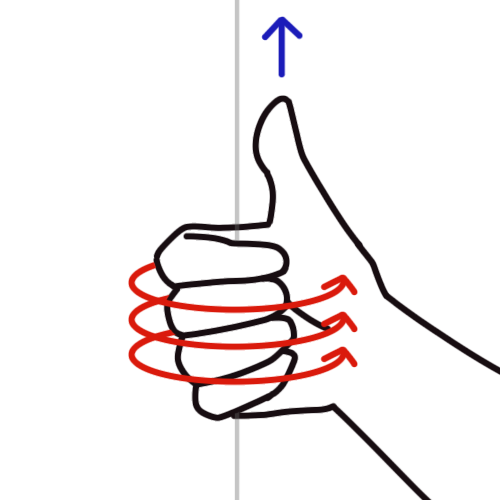
\includegraphics[width=0.7\textwidth]{figures/right-hand-rule.png}
    \caption{The right hand rule for rotation}
    \label{fig:right-hand-rule}
\end{figure}

We note that if we were to invert our hand, so that our thumb points in the opposite direction, then the fingers now curl in the opposite direction relative to the initial axis. Therefore we can imagine if we were to rotate in the negative direction about this inverted vector, we would achieve the same rotation as before. This is to say a positive rotation about some vector is equivalent to a negative rotation about the negation of the vector.\\

This is the reason that quaternions are considered a \socalled{double cover} of 3D rotations, since these two constructions describe the same rotation, but are represented by exactly 2 distinct quaternions, q and -q.
$$ q = \cos{\frac{\theta}{2}} + v\sin{\frac{\theta}{2}} \longspace and \longspace -q = -\cos{\frac{\theta}{2}} - v\sin{\frac{\theta}{2}}$$





%old stuff
%In the context of robot manipulation, reinforcement learning stands as one of the most widely used paradigms. Reinforcement learning allows for a single agent to iteratively improve at a given target task. A reinforcement learning task is characterised by 3 main factors: The set of possible states the agent and environment can be in, the set of actions which the agent is allowed to take, and the reward function which informs the agent how well it has performed.
%While these first two points are often out of our control, defined by the environment setup and the robot respectively, the third point is something problem specific which needs defining. A standard reinforcement learning agent will need a distinct reward function for each individual skill the robot wants to learn. This is a time consuming process and may not even be practical for all tasks.

%\section{Imitation reward function}
%A common solution to this problem is to define the reward function in a manner that is generalisable to other tasks. A popular example is the use of mimicry. In this case the robot is provided a demonstration, either through teleoperation or kinesthetic movement which it remembers as how to perform this skill. The reward function then becomes making the robot copy this demonstration as closely as possible. While this is a good start, if the robot only tries to copy the demonstration, the agent will not be robust to changes in the environment or slightly different problem setups. Consider a demonstration which tells the robot how to pick up a mug. If we were to test the robot by moving the mug but provided it no additional information, the robot would obviously fail to pick up the mug. This is because the robot's reward function is not encoded as \speech{Did I pick up the mug?} because this would be very difficult to formalise. Instead the robot is just asking \speech{Did I follow the demonstration?} which it did. In order to make the agent generalisable to different setups it needs more information.
%Talk about multiple demonstrations and how that method works.
%The problem with this method is that it is still time consuming and could be costly to use the equipment for multiple runs. Furthermore, this method has high variability based on the quality of the demonstrations provided. If the demonstrations are not sufficiently diverse, then the agent may struggle with some problem setups it had not encountered.

%In an attempt to alleviate some of these problems, the paper on mimicGen (reference) poses an algorithm to produce a large dataset of demonstrations from only very few human demonstrations. This drastically reduces the mount of human interaction needed. The paper claims \speech{Agent performance is comparable on 200 MimicGen demos and 200 human demos, despite MimicGen only using 10 source human demos}. What this means is that instead of needing to perform 200 human demos, you only need to perform around 10 without loss in performance. Additionally, mimicGen is specifically designed to create a diverse set of demonstrations, reducing the problem of the agent finding itself in a specific problem setup it doesnt have much information about.

%The One shot imitation papaer (reference) uses an alternative aproach to prevent needing to collect multiple demonstrations at all. Instead of collecting additional information through repeated demonstrations, it saves an image of the problem setup before the demonstration is given which it calls the \speech{context vector} This image is stored along with the single demonstration of the task. This provides the agent the context in which this demonstration was useful. In order to perform the demonstration in a new unseen problem setup, the agent first takes a picture of the new problem setup. This picture is taken using an RGB-D camera. The agent then estimates the pose transformation between the object of relevance in the demonstration image and this new image. Once the agent has estimated the transformation, it can apply this same transformation to the demonstration it was given. By doing so it transforms the demonstration into this new problem setup, wherein the agent can simple imitate the transformed trajectory to complete the task. 